
\subsection{Classification prédictive}

Après ce cuisant echec, nous avons opté pour un changement d'architecture. Nous avons donc recommencé cette fois ci avec
un modèle de classification prédictive. Celà consiste à attribuer une étiquette de classe aux exemples d'entrée. A partir des
connaissances a priori (données et modélisation), le modèle donne une probabilité pour l’événement. De tels modèles sont
appelés modèles de classification. Les modèles prédictifs introduisent une notion de risque; ils ne font pas de prédiction
totalement certaine.

\vspace{1.5cm}

Nous avons tout d'abord défini le premier modèle. Il est composé de 4 couches composées
respectivement de 11 neurones en entrée, de 4 neurones chacunes pour les 2em et 3em couches
et 1 neurone pour la couche de sortie.

Avec cette configuration, nous avons défini un modèle de régression et obtenu
les résultats suivants :

\begin{figure}[!htb]
    \begin{minipage}{0.5\textwidth}
        \centering
        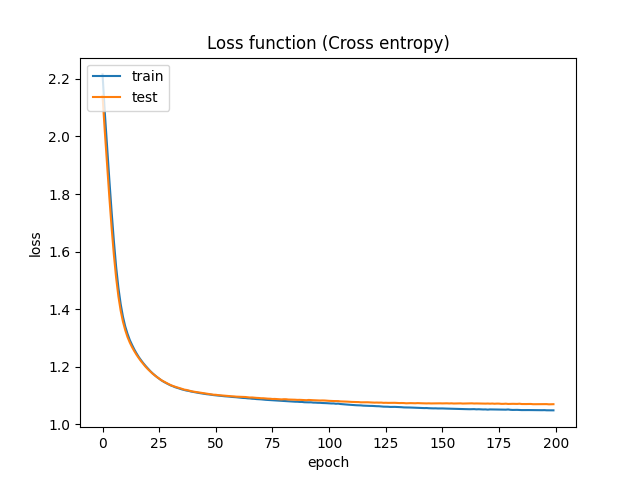
\includegraphics[width=1\textwidth]{../images/11-4-4/Loss_function(Cross_entropy).png}
        \label{fig:11-4-4-10}
    \end{minipage}\hfill
    \begin{minipage}{0.5\textwidth}
        \centering
        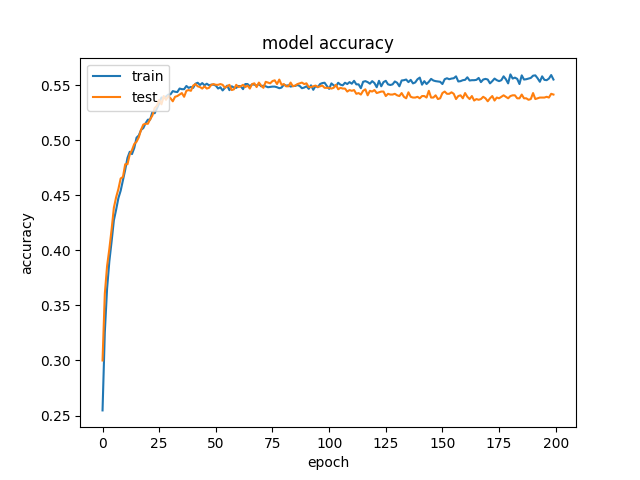
\includegraphics[width=1\textwidth]{../images/11-4-4/model_accuracy(Cross_entropy).png}
        \label{fig:8-4-4-10.2}
    \end{minipage}
    \caption{11-4-4-10}
\end{figure}

Des le debut, on observe une amélioration par rapport aux modèles de régression. Les courbes de
teste et d'entrainement sont maintenant proches mais pas superposées.

Comme pour la regression, complexifions le modèle.

\vspace{1cm}

\begin{figure}[!htb]
    \begin{minipage}{0.5\textwidth}
        \centering
        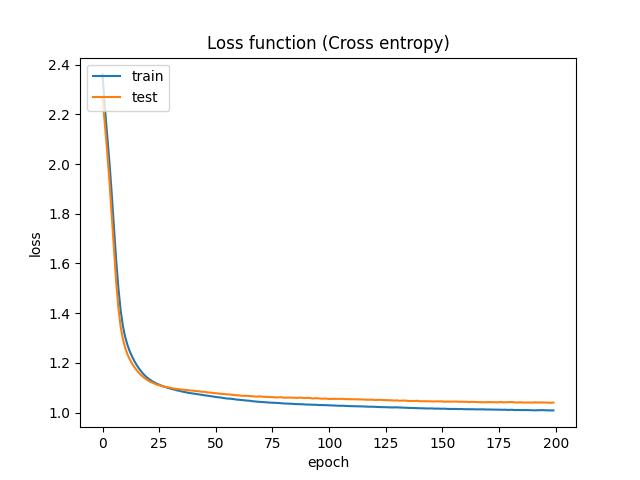
\includegraphics[width=1\textwidth]{../images/11-8-8/Loss_function(Cross_entropy).png}
        \label{fig:11-8-8-10}
    \end{minipage}\hfill
    \begin{minipage}{0.5\textwidth}
        \centering
        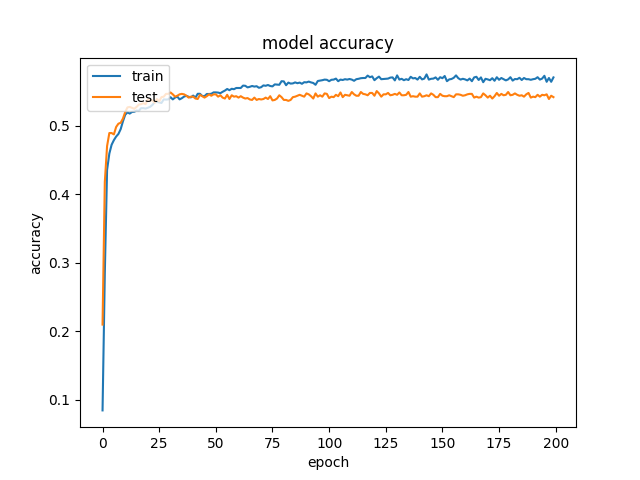
\includegraphics[width=1\textwidth]{../images/11-8-8/model_accuracy(Cross_entropy).png}
        \label{fig:11-8-8-10.2}
    \end{minipage}
    \caption{11-8-8-10}
\end{figure}


\newpage

Les courbes ne semblent pas avoir beaucoup été impactées par le changement de la configuration. Continuons de complexifier le modèle.

\vspace{1cm}

\begin{figure}[!htb]
    \begin{minipage}{0.5\textwidth}
        \centering
        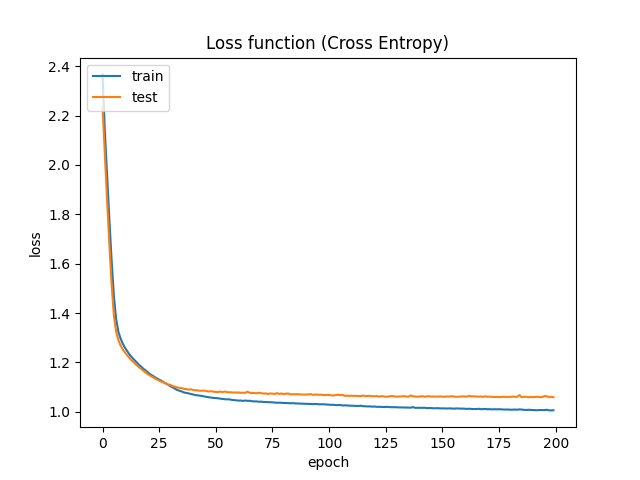
\includegraphics[width=1\textwidth]{../images/11-8-8-8/Loss function(Cross entropy).png}
        \label{fig:11-8-8-8-10}
    \end{minipage}\hfill
    \begin{minipage}{0.5\textwidth}
        \centering
        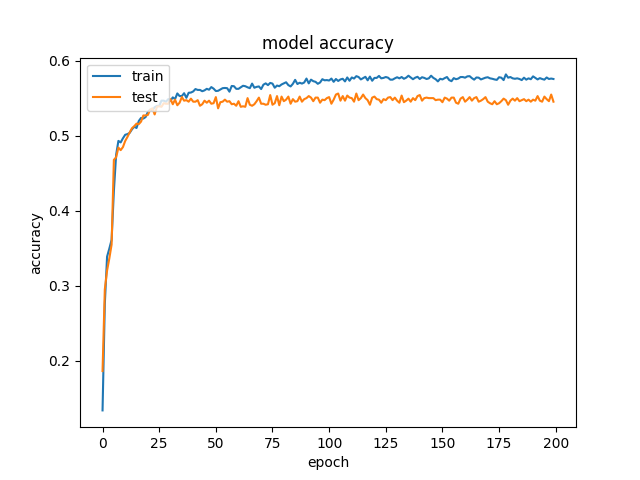
\includegraphics[width=1\textwidth]{../images/11-8-8-8/model accuracy(Cross entropy).png}
        \label{fig:11-8-8-8-10.2}
    \end{minipage}
    \caption{11-8-8-8-10}
\end{figure}

\vspace{1cm}

Contrairement à la régression, le modèle semble déjà converger vers une meilleure généralisation dès 8 neurones par couches.
En effet, on voit bien que les courbles d'entrainement et de teste sont séparées tout en étant suffisement proches pour ne pas créer de
sur-apprentissage.

Dans notre quête de perfection, nous avons donc décidé de continuer de complexifier le modèle en essayant par exemple de rajouter une couche.
Notre nouveau modèle avec 3 couches de  est donc composé de 5 couches composées respectivement de 11 neurones en entrée, de 8 neurones chacunes pour les 2em, 3em et 4em couches

\begin{figure}[!htb]
    \begin{minipage}{0.5\textwidth}
        \centering
        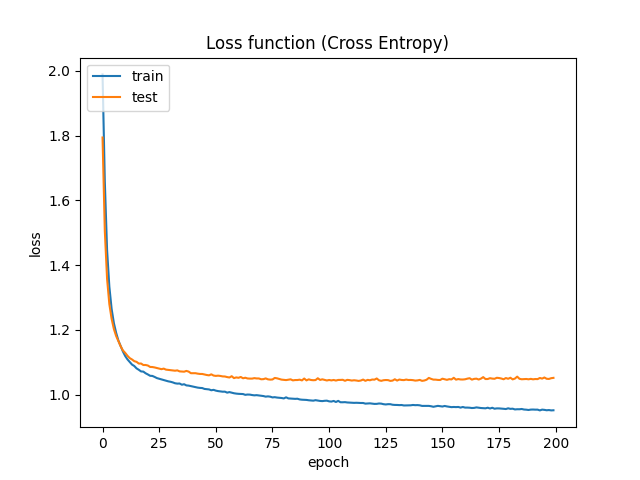
\includegraphics[width=1\textwidth]{../images/11-12-12-12/Loss function(Cross entropy).png}
        \label{fig:11-12-12-10}
    \end{minipage}\hfill
    \begin{minipage}{0.5\textwidth}
        \centering
        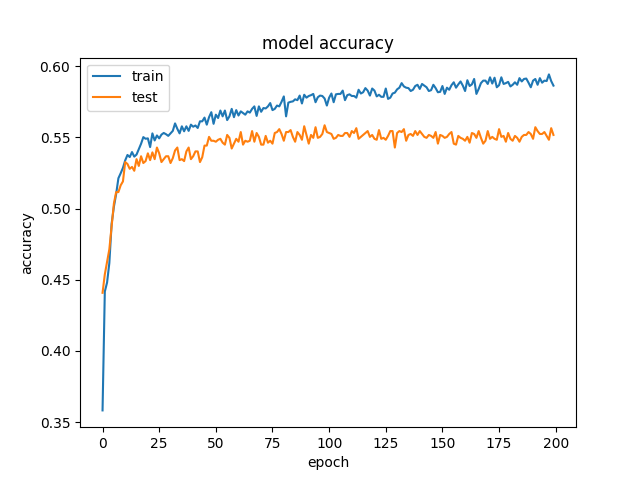
\includegraphics[width=1\textwidth]{../images/11-12-12-12/model accuracy(Cross entropy).png}
        \label{fig:11-12-12-10.2}
    \end{minipage}
    \caption{11-8-8-8-10}
\end{figure}

Malgré tout notre modèle peine à généraliser. Il ne semble pas exéder les 55\% de précision et commence à tendre vers un sur-apprentissage.
Tout comme pour le modèle de régression, nous avons décidé de supprimer les caractéristiques inutiles.
Celà fait, nous avons retenté les mêmes expériences que précédemment.

\vspace{1cm}

\begin{figure}[!htb]
    \begin{minipage}{0.5\textwidth}
        \centering
        \includegraphics[width=1\textwidth]{../images/bonnes_caractéristiques_suppr/8-8-8-8/Loss function(Cross Entropy).png}
        \label{fig:8-8-8-8-10}
    \end{minipage}\hfill
    \begin{minipage}{0.5\textwidth}
        \centering
        \includegraphics[width=1\textwidth]{../images/bonnes_caractéristiques_suppr/8-8-8-8/model accuracy(Cross Entropy).png}
        \label{fig:8-8-8-8-10.2}
    \end{minipage}
    \caption{8-8-8-8-10}
\end{figure}

\begin{figure}[!htb]
    \begin{minipage}{0.5\textwidth}
        \centering
        \includegraphics[width=1\textwidth]{../images/bonnes_caractéristiques_suppr/8-12-12-12/Loss function(Cross Entropy).png}
        \label{fig:8-12-12-12-10}
    \end{minipage}\hfill
    \begin{minipage}{0.5\textwidth}
        \centering
        \includegraphics[width=1\textwidth]{../images/bonnes_caractéristiques_suppr/8-12-12-12/model accuracy(Cross Entropy).png}
        \label{fig:8-12-12-12-10.2}
    \end{minipage}
    \caption{8-12-12-12-10}
\end{figure}

\begin{figure}[!htb]
    \begin{minipage}{0.5\textwidth}
        \centering
        \includegraphics[width=1\textwidth]{../images/bonnes_caractéristiques_suppr/8-20-20-20/Loss function(Cross Entropy).png}
        \label{fig:8-20-20-20-10}
    \end{minipage}\hfill
    \begin{minipage}{0.5\textwidth}
        \centering
        \includegraphics[width=1\textwidth]{../images/bonnes_caractéristiques_suppr/8-20-20-20/model accuracy(Cross Entropy).png}
        \label{fig:8-20-20-20-10.2}
    \end{minipage}
    \caption{8-20-20-20-10}
\end{figure}

\vspace{1cm}

On observe que le modèle avec 3 couches de 8 neurones semble avoir une généralisation avec un bien plus grande marge de progression que
les autres, nous avons donc tenter de lui donner un plus grand nombre d'époch pour l'entrainement.
Avec 2 fois plus d'époch, voici les résultats obtenus :

\vspace{1cm}


\begin{figure}[!htb]
    \begin{minipage}{0.5\textwidth}
        \centering
        \includegraphics[width=1\textwidth]{../images/bonnes_caractéristiques_suppr/8-8-8-8/Loss function(Cross Entropy).png}
        \label{fig:8-8-8-8-10.3}
    \end{minipage}\hfill
    \begin{minipage}{0.5\textwidth}
        \centering
        \includegraphics[width=1\textwidth]{../images/bonnes_caractéristiques_suppr/8-8-8-8/model accuracy(Cross Entropy).png}
        \label{fig:8-8-8-8-10.4}
    \end{minipage}
    \caption{8-8-8-8-10}
\end{figure}

\vspace{1cm}

Finalement, il s'avère que le modèle ne généralise pas suffisement même avec plus de temps d'entrainement.


\newpage